\subsection{part d}
\begin{itemize}
    \item sensitivity function
    $$
    S_G^{G_{cl}} = \dfrac{1}{1+C(s)G(s)}
    $$
    \begin{figure}[H]
        \caption{sensitivity function bode magnitude}
        \centering
        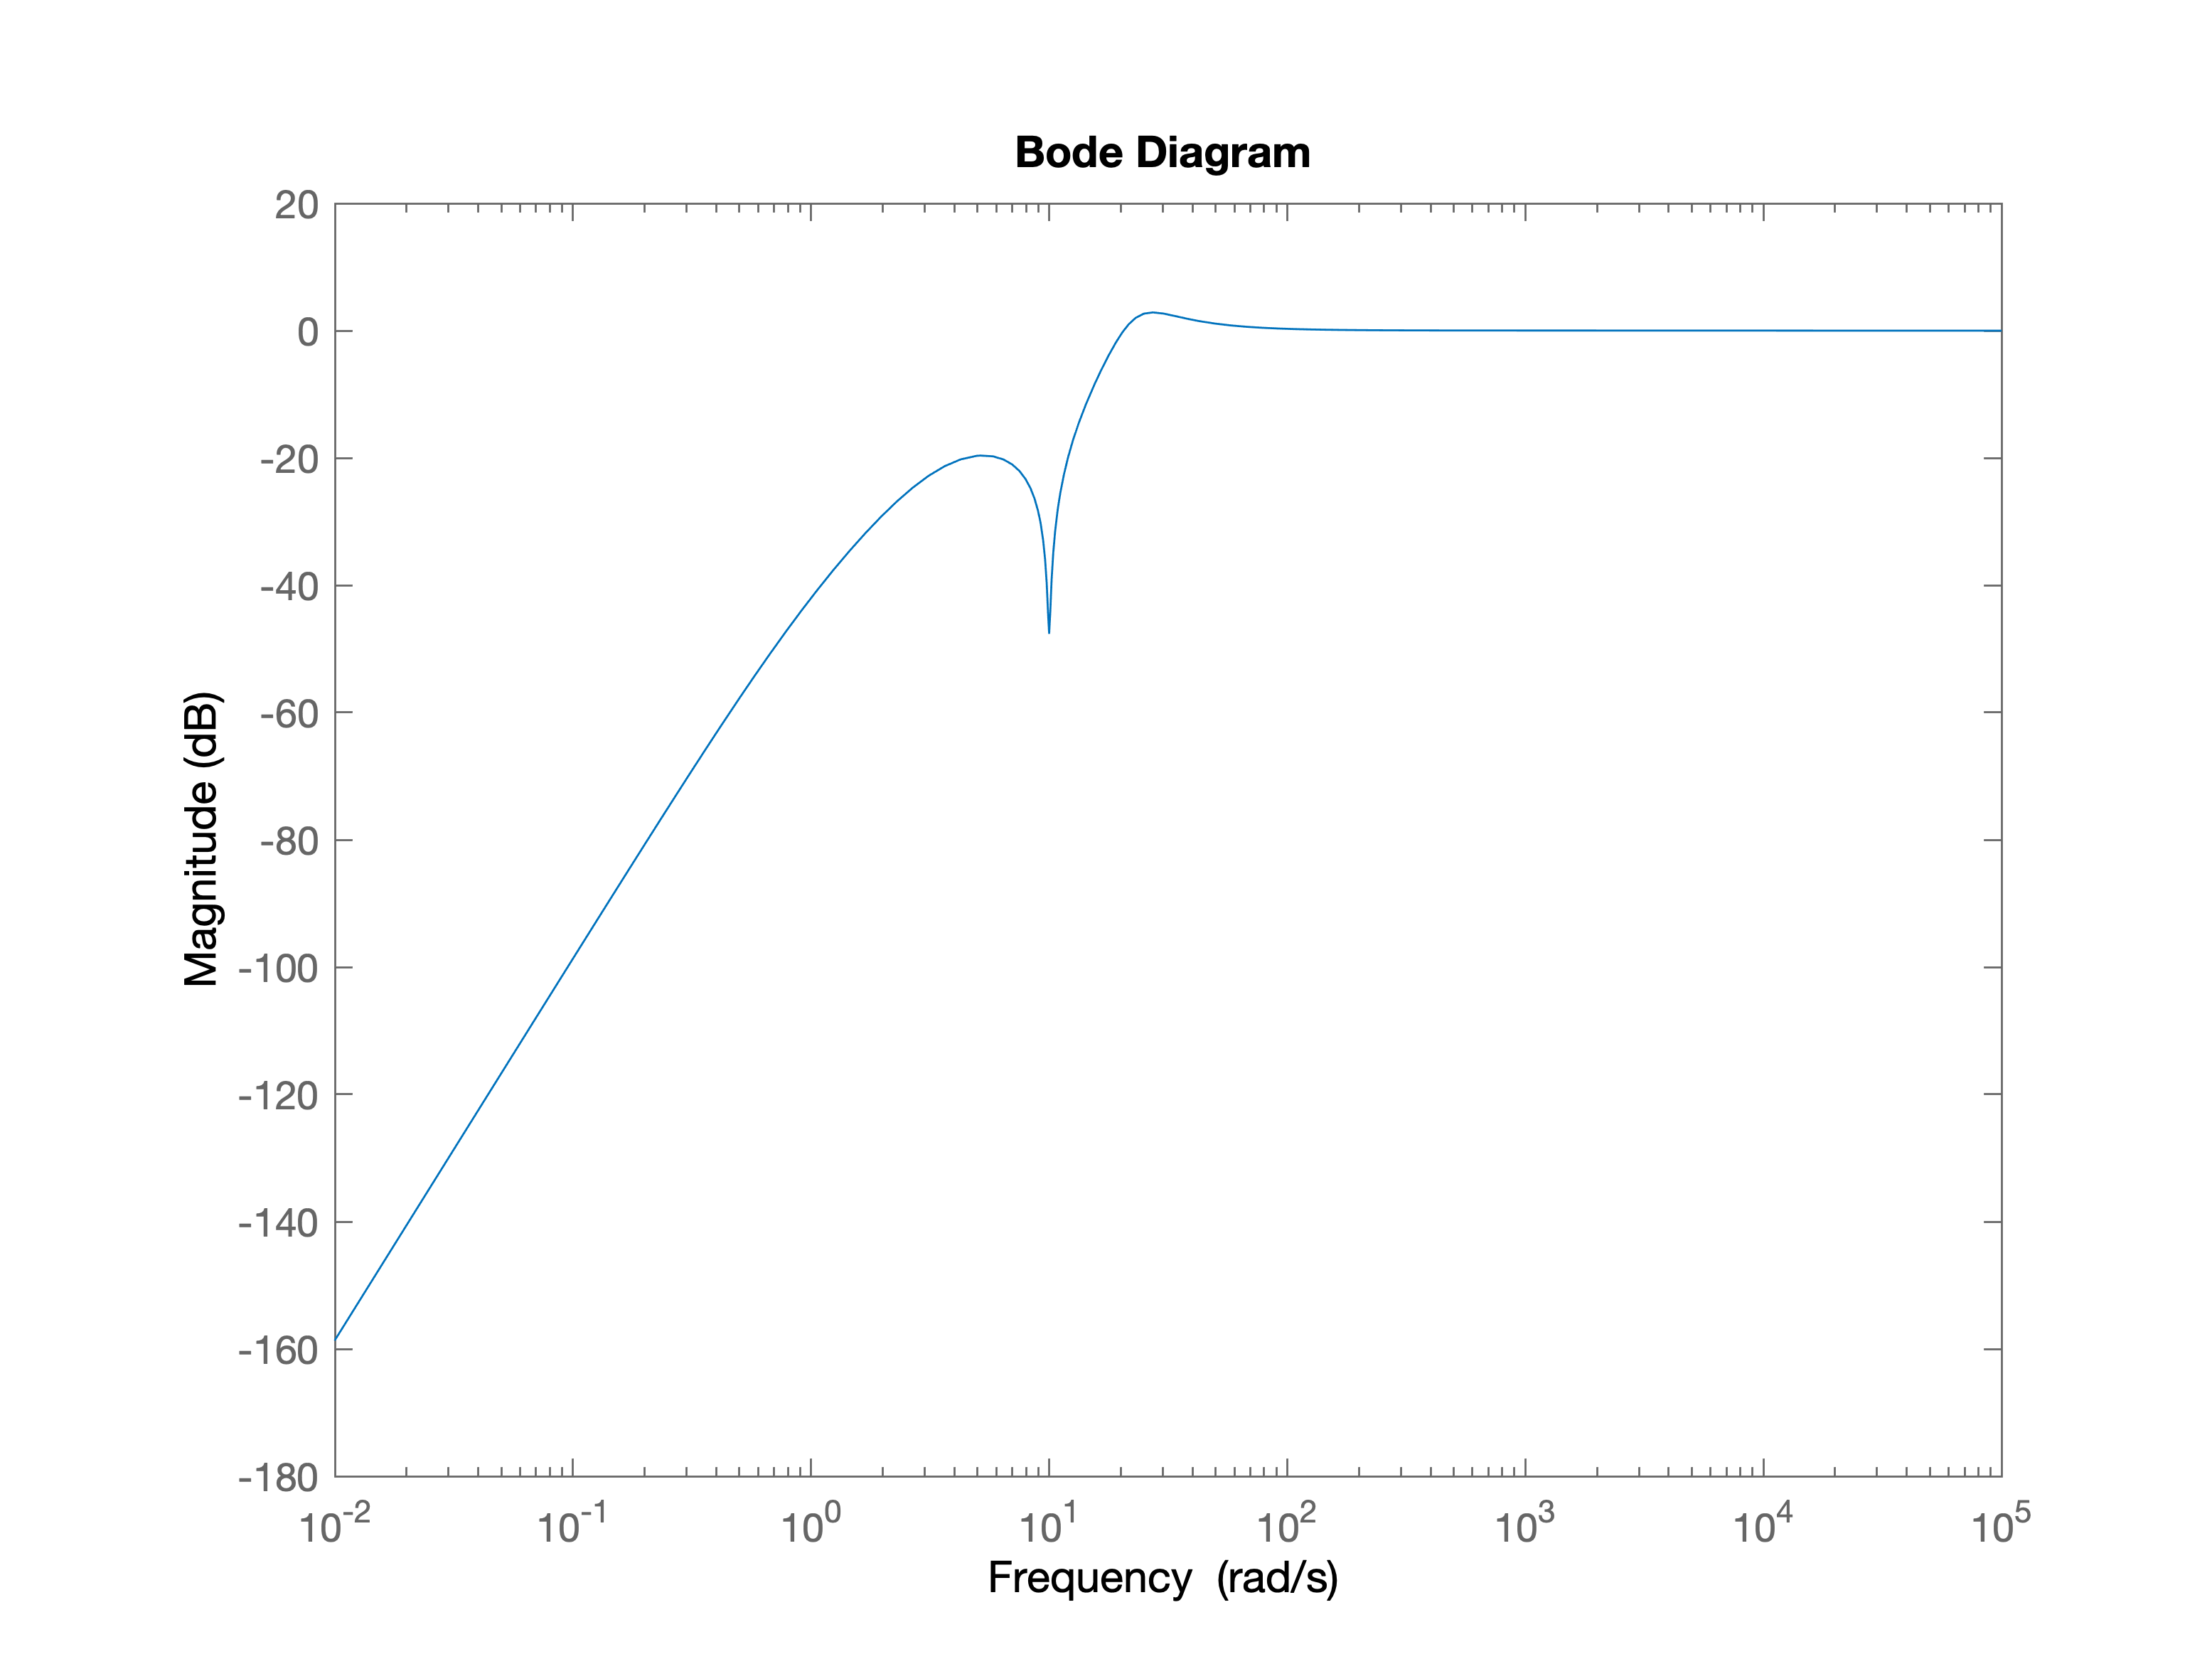
\includegraphics[width=12cm]{../Figure/Q1/Q1_d/sensitivity_func.png}
    \end{figure}
    System sensitivity is very hight at high frequency but low at low frequency.
    \item complementary sensitivity function 
    $$
    S_G^{G_{cl}} = \dfrac{C(s)G(s)}{1+C(s)G(s)}
    $$
    \begin{figure}[H]
        \caption{complementary sensitivity function bode magnitude}
        \centering
        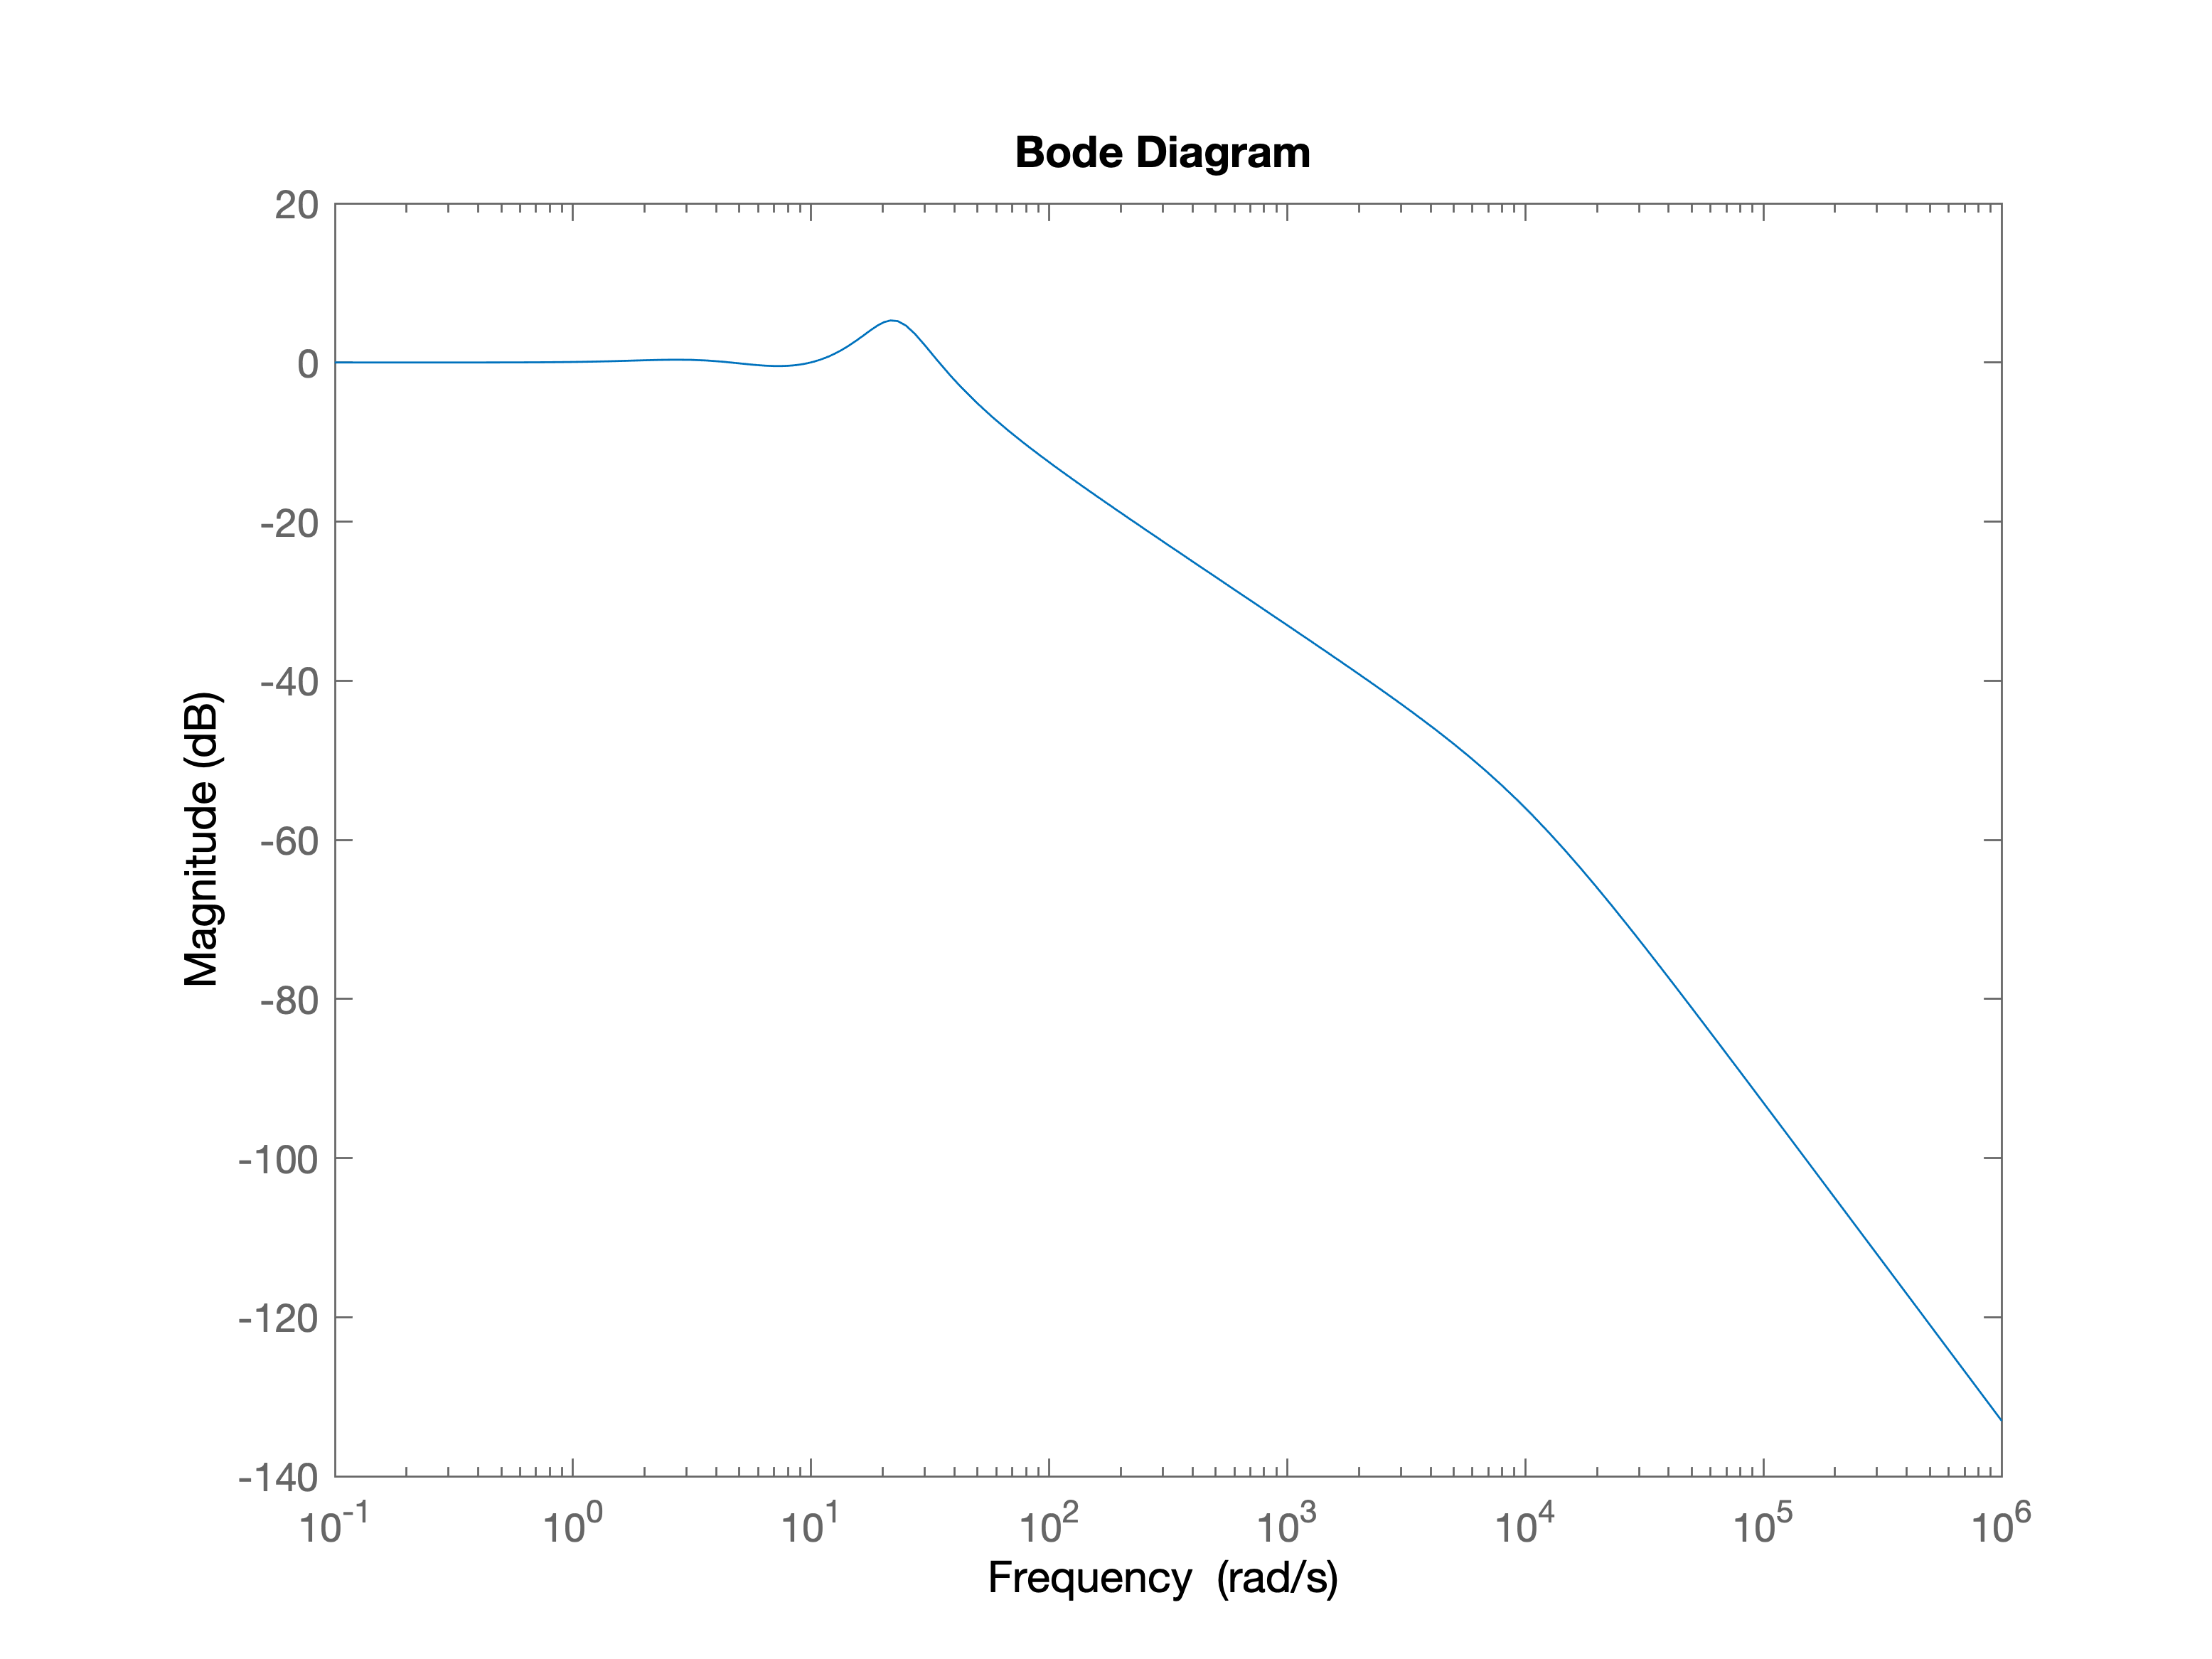
\includegraphics[width=12cm]{../Figure/Q1/Q1_d/com_sensitivity_func.png}
    \end{figure}
    \item Nichols chart for sensitivity function and complementary sensitivity function 
    \begin{figure}[H]
        \caption{nyquist chart}
        \centering
        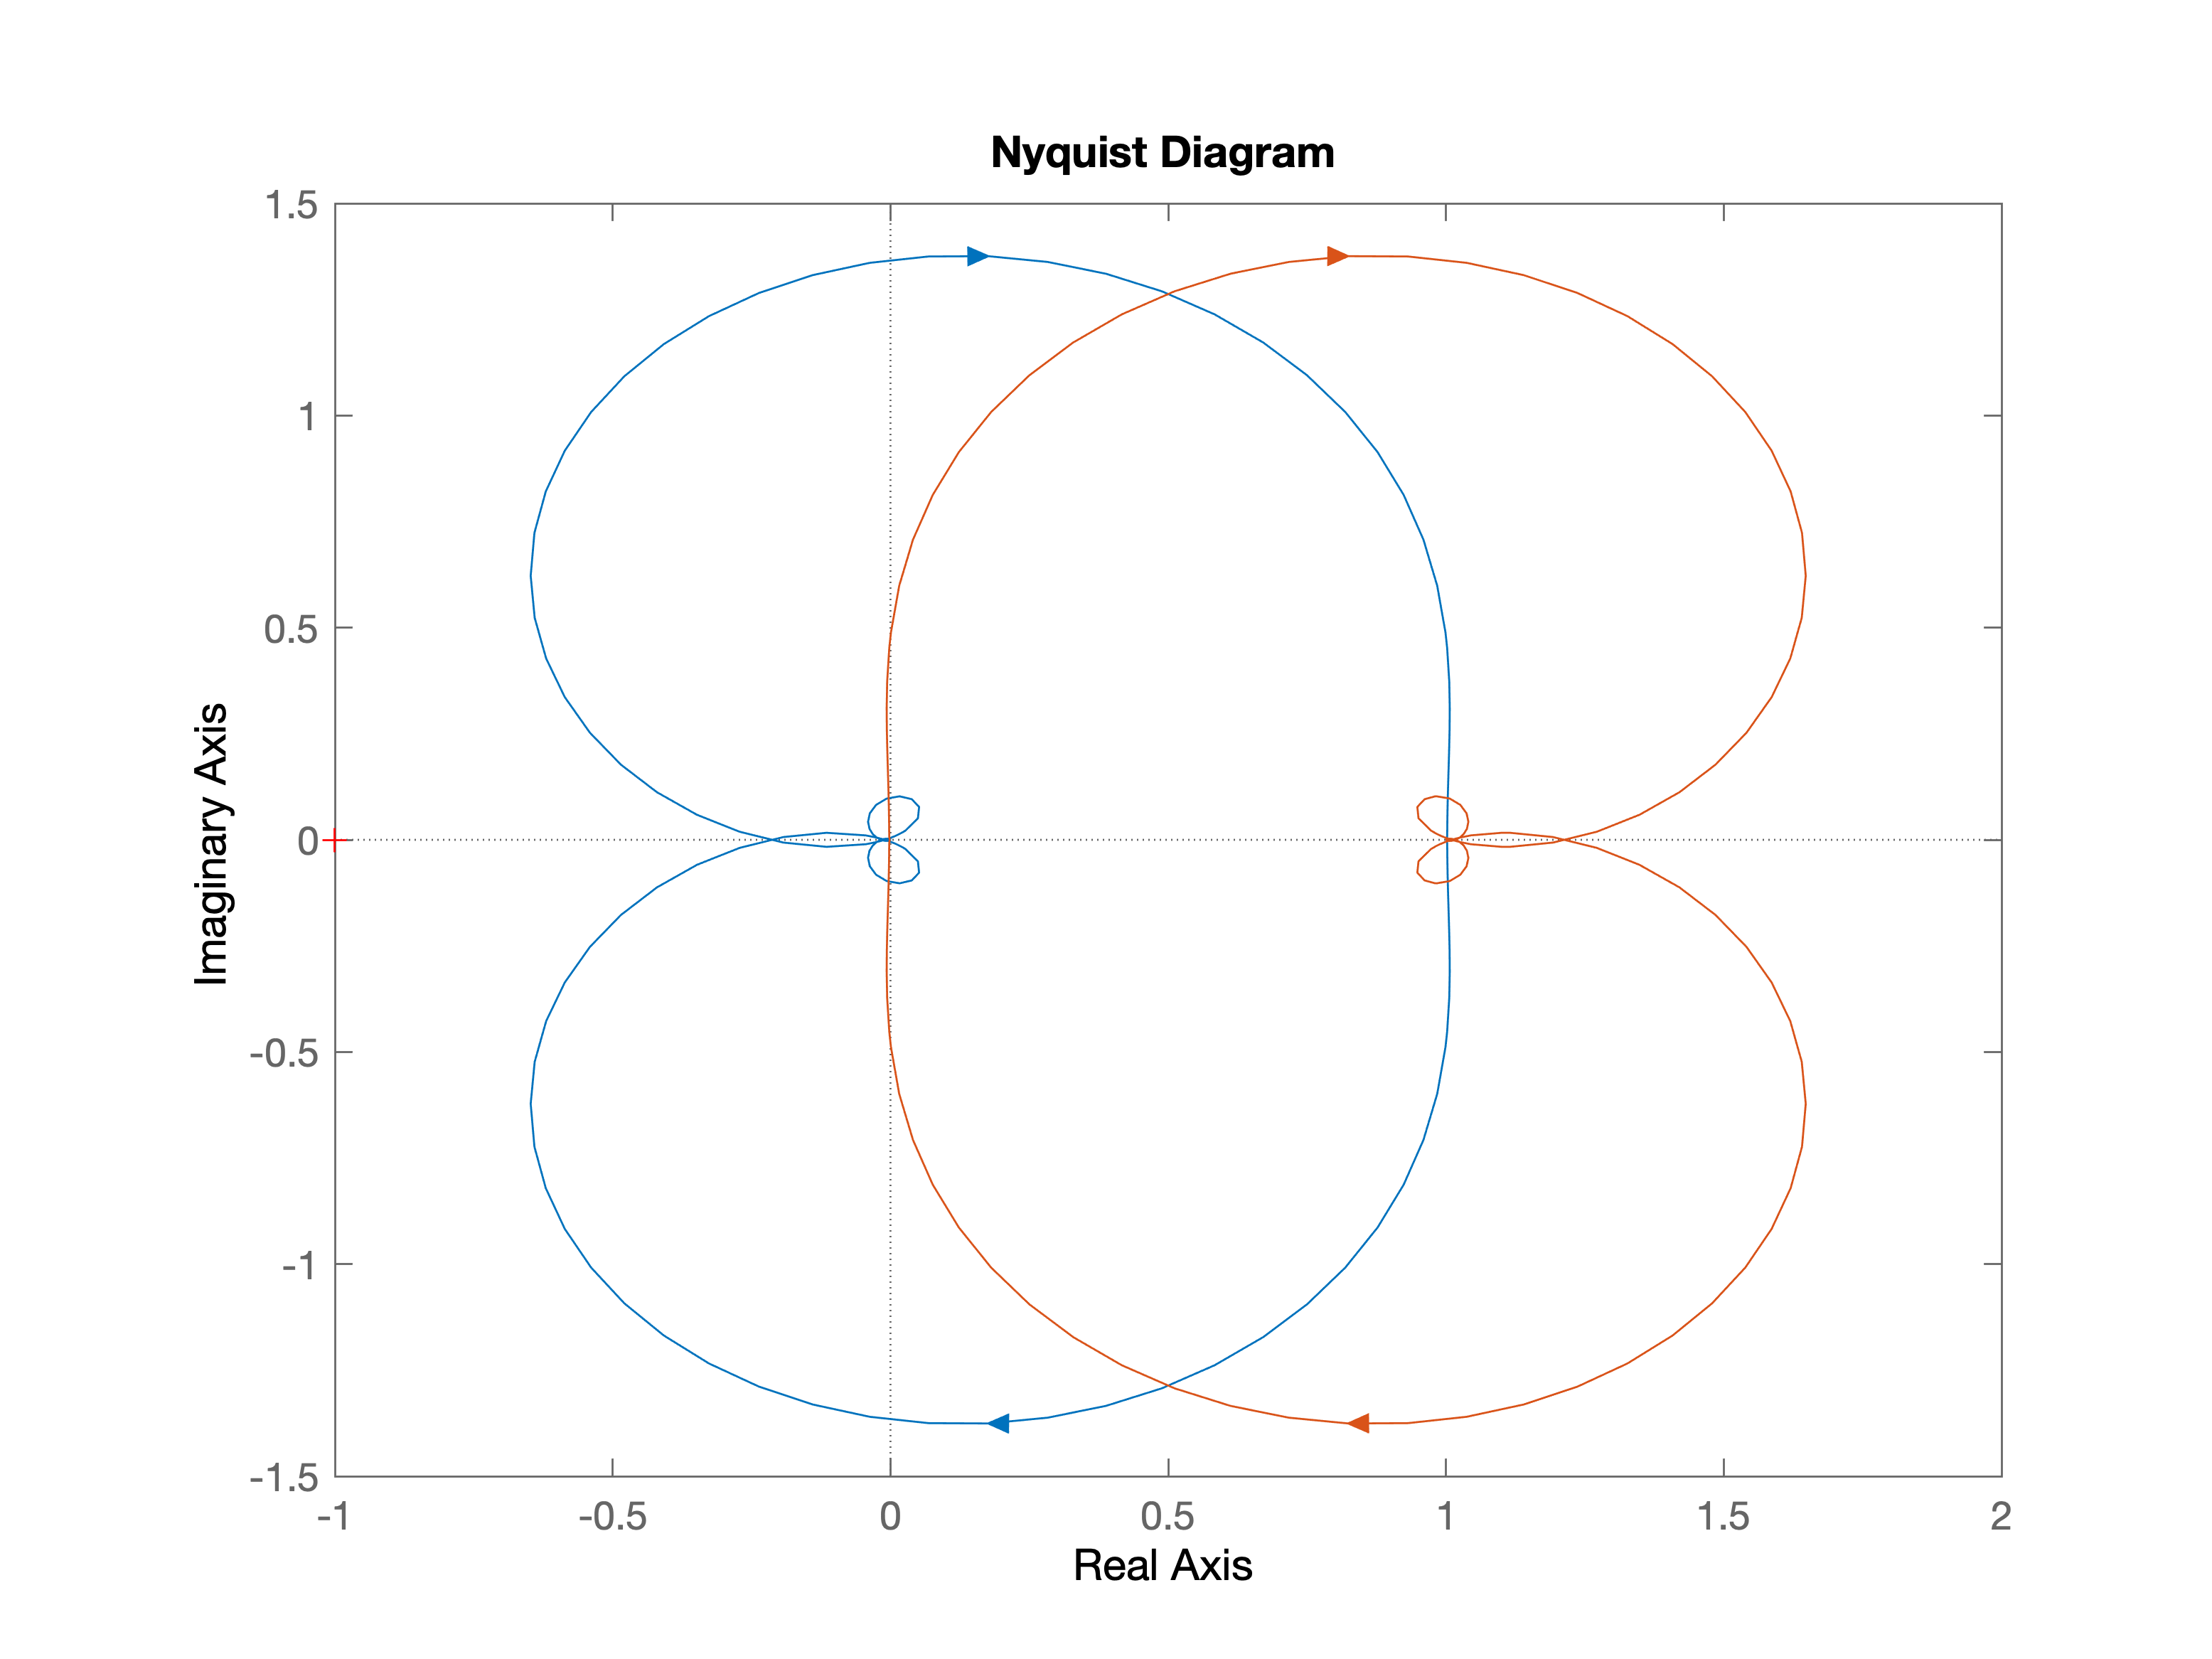
\includegraphics[width=12cm]{../Figure/Q1/Q1_d/nyquist.png}
    \end{figure}
\end{itemize}
